\chapter{Exercise 12}

% ---------------- Exercise 12.1 ----------------
\section{Exercise 12.1}
\subsection{Problem}
Given the following flow graph:
\begin{itemize}
    \item Compute the dominators of all nodes.
    \item Find all back edges in the flow graph.
    \item Find all natural loops defined by each back edge.
\end{itemize}

\begin{figure}[h]
\centering
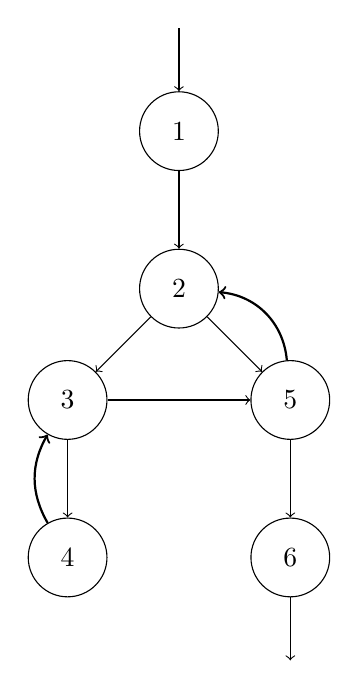
\begin{tikzpicture}[node distance=2cm, auto]
    \node (1) [circle, draw, minimum size=1cm] {1};
    \node (2) [circle, draw, minimum size=1cm, below of=1] {2};
    \node (3) [circle, draw, minimum size=1cm, below left of=2] {3};
    \node (4) [circle, draw, minimum size=1cm, below of=3] {4};
    \node (5) [circle, draw, minimum size=1cm, below right of=2] {5};
    \node (6) [circle, draw, minimum size=1cm, below of=5] {6};

    % External entry and exit
    \draw[->] ([yshift=8mm]1.north) -- (1.north);
    \draw[->] (6.south) -- ([yshift=-8mm]6.south);
    
    % Forward edges
    \draw[->] (1) to (2);
    \draw[->] (2) to (3);
    \draw[->] (2) to (5);
    \draw[->] (3) to (4);
    \draw[->] (3) to (5);
    \draw[->] (5) to (6);
    
    % Back edges
    \draw[->, bend left=30, black, thick] (4) to (3);
    \draw[->, bend right=40, black, thick] (5) to (2);
\end{tikzpicture}
\caption{Flow graph for Exercise 12.1}
\end{figure}

\subsection{Solution}

\subsubsection{Dominators of All Nodes}

We compute the dominators using the standard dataflow algorithm. For each node $n$, $\mathrm{Dom}(n)$ is the set of nodes that dominate $n$.

\begin{itemize}
    \item $\mathrm{Dom}(1) = \{1\}$ \quad (node 1 is the entry and dominates itself)
    \item $\mathrm{Dom}(2) = \{1, 2\}$ \quad (only 1 and 2 dominate 2)
    \item $\mathrm{Dom}(3) = \{1, 2, 3\}$ \quad (1, 2, and 3 dominate 3)
    \item $\mathrm{Dom}(4) = \{1, 2, 3, 4\}$ \quad (1, 2, 3, and 4 dominate 4)
    \item $\mathrm{Dom}(5) = \{1, 2, 5\}$ \quad (1, 2, and 5 dominate 5)
    \item $\mathrm{Dom}(6) = \{1, 2, 5, 6\}$ \quad (1, 2, 5, and 6 dominate 6)
\end{itemize}

\subsubsection{Back Edges}

A back edge is an edge $(u, v)$ where $v$ dominates $u$ in the dominance tree (i.e., $v$ comes before $u$ in a depth-first spanning tree).

Back edges in this flow graph:
\begin{itemize}
    \item Edge $(4, 3)$: Since $3 \in \mathrm{Dom}(4)$, this is a \textbf{back edge}.
    \item Edge $(5, 2)$: Since $2 \in \mathrm{Dom}(5)$, this is a \textbf{back edge}.
\end{itemize}

All other edges $(1,2)$, $(2,3)$, $(2,5)$, $(3,4)$, $(3,5)$, and $(5,6)$ are forward edges.

\subsubsection{Natural Loops}

For each back edge $(u, v)$, the natural loop is the set of nodes that can reach $u$ without going through $v$.

\paragraph{Natural loop for back edge $(4, 3)$:}
\begin{align*}
\text{Loop}_{4 \to 3} &= \{3, 4\}
\end{align*}
This loop includes node 3 (the header) and node 4, since 4 reaches 3 directly via the back edge, and 3 only reaches 4 via the forward edge.

\paragraph{Natural loop for back edge $(5, 2)$:}
\begin{align*}
\text{Loop}_{5 \to 2} &= \{2, 3, 4, 5\}
\end{align*}
This loop includes node 2 (the header), and all nodes that can reach 5 without passing through node 2. Because there is a forward edge $(3, 5)$, node 3 is also included, and then node 4 is included through the back edge $(4, 3)$. Thus the loop is $\{2, 3, 4, 5\}$.



\begin{table}[h]
\centering
\begin{tabular}{|l|l|l|}
\hline
\textbf{Back Edge} & \textbf{Loop Header} & \textbf{Natural Loop} \\
\hline
$(4, 3)$ & 3 & $\{3, 4\}$ \\
\hline
$(5, 2)$ & 2 & $\{2, 3, 4, 5\}$ \\
\hline
\end{tabular}
\caption{Back edges and their natural loops}
\end{table}